\documentclass[12]{article}

\usepackage{gensymb}
\usepackage{float}
\usepackage{float}
\usepackage{booktabs}
\usepackage{multirow}
\usepackage{amsmath}
\usepackage[utf8]{inputenc}
\usepackage[T1]{fontenc}
\usepackage{hyperref}
\usepackage {geometry}
\usepackage {textcomp}
\usepackage[table,xcdraw]{xcolor}

\hypersetup{
    colorlinks,
    citecolor=black,
    filecolor=black,
    linkcolor=black,
    urlcolor=black
}

\setlength{\oddsidemargin}{0.25 in}
\setlength{\evensidemargin}{-0.25 in}
\setlength{\topmargin}{-0.6 in}
\setlength{\textwidth}{6.5 in}
\setlength{\textheight}{8.5 in}
\setlength{\headsep}{0.75 in}
\setlength{\parindent}{0 in}
\setlength{\parskip}{0.1 in}

%\counterwithin{figure}{subsection}
\usepackage{chngcntr}
\usepackage{graphicx}
\usepackage[inkscapeformat=pdf,inkscapelatex=false]{svg}
\graphicspath{ {./figs/} }

\begin{document}
\begin{titlepage}
\newcommand{\HRule}{\rule{\linewidth}{0.5mm}}
\setlength{\topmargin}{0 in}
\begin{center}

\begin{figure}[!h]
\centering

\includegraphics [width=0.3\textwidth]{eelogo.png}
\end{figure}

\vspace{10mm}
\Huge{MIDDLE EAST TECHNICAL UNIVERSITY}\\
\vspace{5mm}
{\LARGE ELECTRICAL \& ELECTRONICS ENGINEERING}\\
\vspace{4mm}
\LARGE{Şönt A.Ş.}\\

\HRule\\[0.4cm]
\textsc{\Large{EE464 - STATIC POWER CONVERSION II}}\\
\textsc{\Large{Hardware Project - Flyback Converter\\}}
\textsc{\Large{Simulation Report\\}}
\HRule\\[0.4cm]

\vspace{3mm}

\end{center}
\begin{minipage}{1\textwidth}
		\begin{flushleft}
			\large
			Orhun  \textsc{Taşoğlu - 2094506}\\
			Fahri \textsc{Türedi - 2167435}\\
			Nurettin \textsc{Çavuş - 2094878}
			
		\end{flushleft}
	\end{minipage}

\vspace{10mm}
\begin{center}
\large{23.03.2020}
\end{center}
\end{titlepage}

\tableofcontents
\newpage
\section{Introduction}

One of the most commonly used circuit to perform DC-DC conversions are Switching Mode Power Supplies (SMPS). To provide a safer output and to comply with international standards isolation of output from the input side is required, especially in grid-connected applications. There are two main topologies of the dc-dc converters with galvanic isolation which means there is no electrical contact between two sides are the Flyback Converters and Forward Converters. These topologies provide isolation thanks to the isolation transformer placed between the two sides. The isolation transformer also provides larger bandwidth or operation range on the voltage transfer capabilities by adjusting the primary to secondary turns ratio. Hence, these topologies reduce the weight of the duty ratio on the voltage transfer capability by having the turn ratio of the transformer to make the most of the work. 

In this report, fundamental points of our design, parameter calculations. simulation results and key components for building the Flyback Converter topology are explained. First of all, the reasoning behind the topology selection is presented. Then, the design methodology of the Flyback Converter is given with the design goals and parameter calculations in the following part. The magnetic design of the transformer is also be explained in detail. Depending on the design selections and computed parameters, the simulation results of the constructed topology is presented in the Simulation Results part of the report. Finally, the component selections for the semiconductor devices are included according to the maximum current and voltage stresses over them, which are computed by the analytical calculations and observed during the simulations. The magnetic core selection for the transformer is can be found in that part of the report too. Furthermore, the appropriate cable selection both for the primary and secondary sides of the transformer is done considering the effects like the skin effect and the proximity effect together with the maximum currents flowing through the transformer windings.

\section{Topology Selection}

\textbf{Selected Topology: FLY\#1}

We, as Şönt A.Ş., selected the Flyback Converter topology FLY\#1 over Flyback Converter options and Forward Converter topology for a number of reasons. First of all, it includes less number of components compared to the Forward Converter topology. Hence, the cost is reduced compared to the Forward Converter topology. Another reason is that it does not require an output filter inductor, which makes the magnetic design phase easier compared to the Forward Converter topology. As a result, there is no need for a second core selection and extra magnetic design for an output filter inductor. In terms of these aspects, the Flyback Converter topology is the simplest topology among the other options. \par Furthermore, the voltage gain control of the Flyback Converter topology in DCM operation is easier than that in the Forward Converter topology. As a result, the current mode control and the voltage mode control of the Flyback Converters can be made in DCM operation, which also helps to reduce the current stress over the MOSFET and the diode during switching since the switching is done when the current is equal to zero. Zero current switching also eliminates the reverse recovery losses over the output rectifier diode. Furthermore, the DCM operation allows switching the MOSFET when the voltage across the drain to source terminals of the MOSFET is approximately equal to the input voltage. This greatly reduces the switching losses of the converter since the switching losses are proportional to the square of the drain to source voltage of the MOSFET. \par The availability of DCM operation also enables the valley switching operation, which further decreases the switching losses by making it possible to switch the MOSFET while the drain to source voltage is at its minimum below the input voltage. This operation requires frequency modulation (FM) controlled by a controller. Since we found the UCC28740 to be widely available, inexpensive and capable of completing the tasks given in the project, we decided to build our Flyback Converter around it. The EMI effects are also reduced with the valley switching operation.  All in all, these operation modes make the Flyback Converter topology obtain a higher efficiency than Forward Converter topology. One another advantage of the availability of DCM operation is that it helps to reduce the required inductance value for the transformer, which helps to reduce the transformer size and weight. If we evaluate the two topologies in terms of voltage stress over the switching MOSFET, the voltage stress over the switching MOSFET in Flyback Converter topology is less than that in the Forward Converter topology. These points and considerations conclude our selection of Flyback Converter topology over Forward Converter topology.

Now, the final topology selection among the three possible Flyback Converter topology options FLY\#1, FLY\#2 and FLY\#3 will be explained.

If we compare the Flyback Converter topology options FLY\#1, FLY\#2 and FLY\#3 in itself, we did not want to work with AC input voltage since it would require an extra input full bridge rectifier together with an very large filter capacitor at the rectifier output. This eliminated the option FLY\#3 for us. Then, between FLY\#1 and FLY\#2, we selected the FLY\#1 option since its output voltage is higher than that of FLY\#2 option. This makes the average output current in FLY\#1 less than that in the FLY\#2, which helps to increase the efficiency in the FLY\#1 option compared to FLY\#2 option. Also, the current ripples and maximum current ratings will be smaller in FLY\#1 due to smaller average output current. In addition, the higher output voltage for the same output voltage ripple limit of 4\% helps to choose the output filter capacitor smaller in FLY\#1 option, which reduces the filter size. For these reasons, we selected the FLY\#1 option.
\section{Flyback Converter Design}

\begin{figure}[H]
\begin{center}
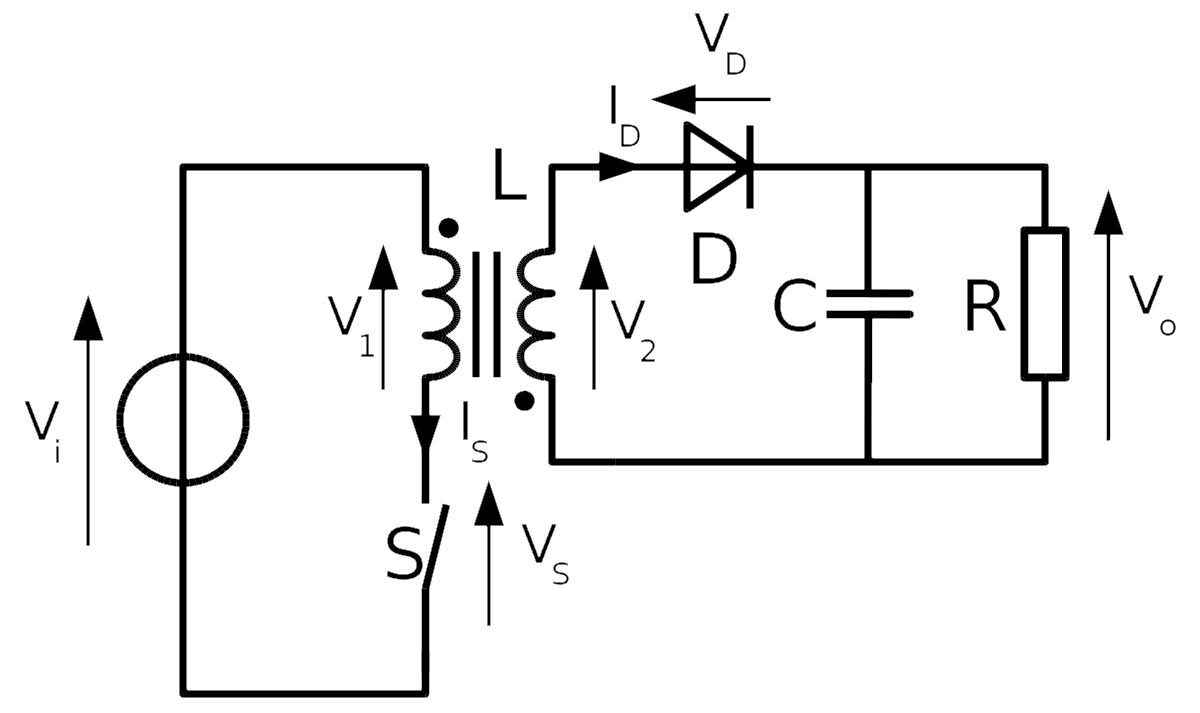
\includegraphics[width=0.6\textwidth]{flybacktop.png}
\caption{Ideal Flyback Converter}
\label{fig:flybacktop}
\end{center}
\end{figure}
An ideal flyback converter topology is given in Figure \ref{fig:flybacktop}. It is a galvanically isolated DC-DC converter with a special feature. That special feature is using the magnetizing inductance of the transformer as an energy storage device, instead of a separate circuit component, which helps reduce the cost, volume and mass of the converter. For our hardware project, we will build a Flyback Converter with extra features to establish the flexibility and performance required to achieve the main requirements and collect bonus points from the Hardware Project. 
\par Our circuit's main controller is UCC28740 by Texas Instruments. It can achieve both current mode and voltage mode control by taking feedback from input and output sides. For UCC28740 to perform properly, the rest of the circuit should be set to achieve DCM operation at all times. UCC28740 can achieve valley switching, which means it will try to switch the MOSFET at the lowest possible voltage than the primary voltage to increase the efficiency. Those voltage levels are called valley points which are bottoms of the voltage swing at the primary, as seen in Figure \ref{fig:valleyswitch}. The lower voltage level is seen because of the ringing when primary current reaches zero. This kind of Flyback Converter called Quasi-Resonant Flyback Converter.

\begin{figure}[H]
\begin{center}
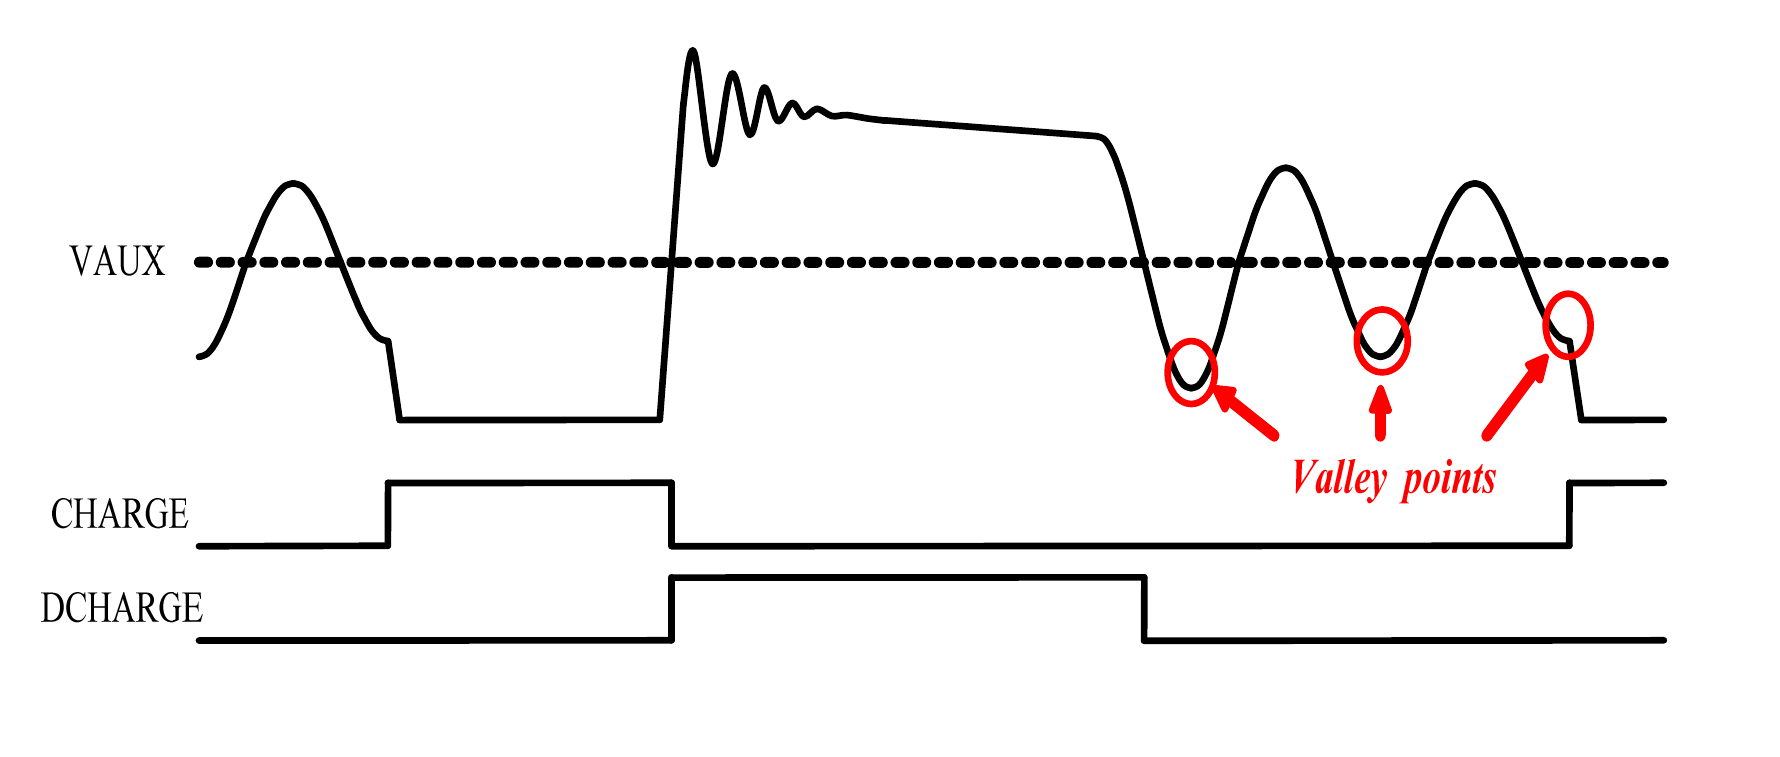
\includegraphics[width=0.6\textwidth]{valleyswitch.png}
\caption{Vallet Points of a Quasi-Resonant Flyback Converter}
\label{fig:valleyswitch}
\end{center}
\end{figure}

To be able to handle synchronous switching, UCC24636 by Texas Instruments will be used at the secondary side. The reference design for the mentioned ICs is given in Figure \ref{fig:refdesign}.

\begin{figure}[H]
\begin{center}
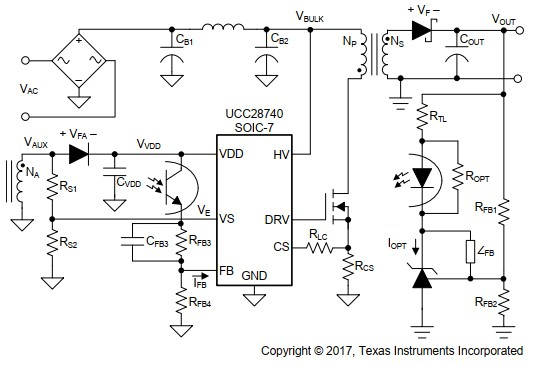
\includegraphics[width=0.6\textwidth]{refdesign.jpg}
\caption{Reference Flyback Converter Design with UCC28740}
\label{fig:refdesign}
\end{center}
\end{figure}


\subsection{Design Goals}
Complying with the specifications given in the project description, Table \ref{tab:specs} is prepared as a summary. Our design must accomplish the given performance measures. In addition to these, the circuit must employ a closed-loop control. Furthermore, to maximize the functionality and gain bonus points we aimed to go for each positive bonus parts described.
\begin{table}[H]
\centering
\caption{Project Specifications}
\begin{tabular}{|c|c|c|c|c|c|}
\hline
\multicolumn{2}{|c|}{\textbf{Paremeter}}   & \textbf{Min}          & \textbf{Typical}      & \textbf{Max}          & \textbf{Unit}         \\ \hline
\multicolumn{2}{|l|}{\textbf{INPUT}}       & \multicolumn{1}{l|}{} & \multicolumn{1}{l|}{} & \multicolumn{1}{l|}{} & \multicolumn{1}{l|}{} \\ \hline
$V_{in}$  & Input Voltage                       & 24                    & 36                    & 48                    & VDC                   \\ \hline
\multicolumn{2}{|l|}{\textbf{OUTPUT}}      &                       &                       &                       &                       \\ \hline
$V_{out}$ & Output Voltage                      & 14.4                  & 15                    & 15.6                  & VDC                   \\ \hline
$I_{out}$ & Output Current                      & -                     & 3.75                  & -                     & A                     \\ \hline
$P_{out}$ & Output Power                        &                       & 60                    &                       & W                     \\ \hline
     & Line Regulation                     &                       &                       & 2                     & \%                    \\ \hline
     & Load Regulation                     &                       &                       & 2                     & \% 
     \hline
\label{tab:specs}
\end{tabular}
\end{table}
\subsection{Parameter Calculations}
\subsubsection*{Duty Cycle, Turns Ratio, Primary Inductance, Peak Primary Current}
Since the target maximum switching frequency imposed by the limitations of our controllers, it is designated as 45 kHz. $D_{MAGCC}$ is defined as `The secondary diode conduction duty-cycle limit in CC mode, 0.425. which is a device parameter to make sure the transformer is demagnetized and DCM is established. Assuming 500 kHz as the DCM resonance frequency, the times it takes to reach the first valley of $V_{DS}$, $t_R$ should be substracted so that valley switching can be made possible too. To find the maximum duty cycle for constant CCM operation,
\begin{align*}
D_{MAX}&=1-D_{MAGCC}-f_{MAX}\times\frac{t_R}{2}\\
D_{MAX}&=1-0.425-45kHz\times \frac{2 \mu s}{2}=0.53
\end{align*}
\par Since $D_{MAX}$ is known, maximum primary to secondary turns ratio can be determined with the following equation:
\begin{align*}
    N_{PS,MAX}=\frac{D_{MAX} V_{DC,min}}{D_{MAGCC}(V_{O}+v_F})=\frac{0.53\times 24}{0.425*(15.7)}=1.906
\end{align*}

Since the voltage at the current sense feedback pin of the controller, $V_CST$ is limited, first we need to determine de $R_{CS}$ to limit the the primary peak current,$I_{PP}$.
\begin{align*}
    R_{CS}&=\frac{V_{CCR}N_{PS}}{2I_{O}}\sqrt{\eta_{transformer}}=74.3m\Omega\\
    I_{PP,MAX}&=\frac{V_{CST,MAX}}{R_{CS}}=\frac{0.773}{0.0746}=10.4A
\end{align*}
Where $V_{CCR}$ is a device parameter called constant-current regulation factor and is equal to 330mV.
To compansate the voltage ripples on the input capactiors, a factor of 0.6 is used. 

%\begin{align*}
%    I_{PPK}=\frac{2P_{out}}{\eta V_{in,min}\sqrt{2}\times 0.8D_{MAX}}=\frac{2\times 60W}{0.85\times %24\sqrt{2}\times 0.6\times 0.53}=13.08A
%\end{align*}


\par To ensure enough energy can be stored in the transformer and DCM operation is established, primary inductance should be specified properly It should be noted that the transformer will cause losses so they need to taken into consideration too. Assuming \% efficiency, magnetizing inductance is calculated.
\begin{align*}
    L_P=\frac{2(V_O+V_F)I_O}{\eta _{transformer}I_{PP,MAX}^2f_{MAX}}=\frac{2\times 15.7\times 4}{0.9\times 10.4^2\times f_{MAX}}=28.67\mu H
\end{align*}
Lastly, since we will need an auxiliary winding to power the controller to sense the primary voltage and utilize low voltage lockout, turns ratio of it should be calculated too. Assuming the lockout voltage to be 15V, and auxiliary diode voltage drop to be 0.5 Volts. Lastly, the upper limit for auxiliary to secondary turns ratio is calculated according to the lowest supply voltage of the controller, $V_{DD,off}$
\begin{align*}
N_{AS,MAX}&=\frac{V_{DD,min}+V_{FA}}{V_O+V_F}=\frac{7.75+0.5}{15+0.7}=0.525\\
N_{PA,MAX}&=\frac{1.9}{0.525}=3.62
\end{align*}

\subsection{Transformer Parameter Verification}
To be able to choose our components properly, the stresses on them should be calculated to make an informed decision. Turns ratio of the transformer affects the peak voltages on the rectifiers. Also, demagnetization and MOSFET on times are should be verified so that the values are in the internal timing limits of our controller.
Reverse voltages on primary and secondary rectifiers are,
\begin{align*}
V_{Reverse,secondary}&=\frac{V_{IN,MAX\sqrt{2}}}{N_{PS}}+V_{O,MAX}=77.8V\\
V_{Reverse,primary}&=\frac{V_{IN,MAX}}{N_{PA}}+V_{VDD}=23.25V
\end{align*}
For MOSFET $V_{DS}$ peak voltage calculation;
\begin{align*}
    V_{DS,peak}=V_{IN,MAX}+(V_O+V_F)N_{PS}=97V
\end{align*}
To find our circuits ON time and Demagnetization times,
\begin{align*}
t_{ON,min}=\frac{L_P}{V_{IN,MAX}}\frac{I_{primary,MAX}}{4}=1.51\mu s\\
t_{Dmag.Min}=\frac{t_{ON,min}V_{IN,MAX}}{N_{PS}(V_O+V_F)}=2.9\mu s
\end{align*}
The minimum required ON time for our controllers is indicated as 280 nS and minimum Demagnetizing time is specified as 2.4 $\mu$S. Both criteria are satisfied and our circuit can operate in nominal conditions.
\subsection{Magnetic Design}
Firstly, the shape of the transformer core is selected as an E-core. Since E-cores can be winded better than toroid cores. To have enough turn numbers on both primary and secondary side, KOOL MU 2510 E CORE(00K2510E090) is selected. Cross-section area of the core is important for turn numbers and core area of the KOOL MU 2510 E CORE is small enough to have 10 turns on the primary side. Parameters of the chosen E-core is given below;
\begin{align}
    A_e &= 35mm^2(Cross Section Area)\\ l_e &= 48.5 mm (Path Length) \\\mu_c &= 90 (Relative Permeability) \\ B_c &= 1 T (Saturation Flux Density) \\ Weight &= 5.9 g and V_e=1870 mm^3 (Volume) 
\end{align}
According to chosen core secondary turn numbers was calculated.
\begin{align}
    N_S&=\frac{L_P\times I_{peak}}{n\times B_m \times A_e}\\
    N_S&=\frac{28.67\times 10^{-6} \times 10.8 }{1.9 \times 1 \times 35 \times 10^{-6}}=5.2 turns
\end{align}
Ratio of the primary turn numbers to secondary turn numbers is calculated, so primary turn number is given below;
\begin{align}
    N_P= n\times N_S = 1.9 \times 5.2 = 10 turns
\end{align}
In this flyback converter design, UCC28740 analog controller is chosen to control the output voltage and current. To supply V$CC$(7.75V) to UCC28740 analog controller, there is required auxiliary winding come from the transformer. The turn number of the auxiliary winding is calculated below;
\begin{align}
    N_{VCC}= \frac{V_{CC}}{V_O+V_F}\times N_S = \frac{7.75}{12+0.7}\times N_S= 3 turns
\end{align}
There is a core gap on the E-core. Core gap is crucial because magnetic flux intensity can be controlled by the core gap. If there is smaller gap than required, the core can be saturated and transformer could not work properly. Also the other components of the flyback converter can be damaged due to overload. Required core gap is calculated to have optimum magnetic design. Calculation of the core gap is given below;
\begin{align}
    gap=\frac{\mu_0\times N_P{^2}\times A_e }{L_P}-\frac{I_e}{\mu_c}=\frac{1.256\times 10^{-6}\times 10{^2}\times 35\times 10^{-6}}{28.67\times 10^{-6}}-\frac{48.5\times 10^{-3}}{90}=1.35\times 10^{-3}m
\end{align}
To check the calculated values given equations is done. Magnetic flux intensity is crucial, since if it is higher than the saturation level of the core, saturation level of the chosen core is 1 Tesla.
\begin{align}
    B=\frac{\mu_0\times N_P\times I_P}{\frac{I_e}{\mu_c}+gap}&=\frac{1.256\times 10^{-6}\times 10\times 10.8}{\frac{48.5\times 10^{-3}}{90}+3.85\times 10^{-3}}=0.95\\
    V_r&=\frac{N_P}{N_S}\times (V_O+V_F)=24.13 V
\end{align}
0.95 Tesla is lower than saturation level of the core so it is acceptable. Also duty ratio must be lower than 0.53. To check duty ratio of the design, D is calculated below;
\begin{align}
    D=\frac{V_r}{V_r+V{_dc(min)}}=0.5
\end{align}


\section{Simulation Results}
The designed converter topology is simulated in Simulink to verify desired functioning of the circuit.

For simplicity, the controller topology and feedback mechanisms are not included in the circuit schematic of the simulation model. Furthermore, the semiconductor devices and filter capacitors and inductors are taken ideal without voltage drops and ESR values.

In order to verify the operation of the circuit, we simulated the converter at its two extreme boundary points for input voltage of $ V_{in} = 24\;V $ and $ V_{in} = 48\;V $.

The Simulink simulation model of the Flyback Converter circuit is given in Figure \ref{fig:schematic}.

\begin{figure}[H]
\begin{center}
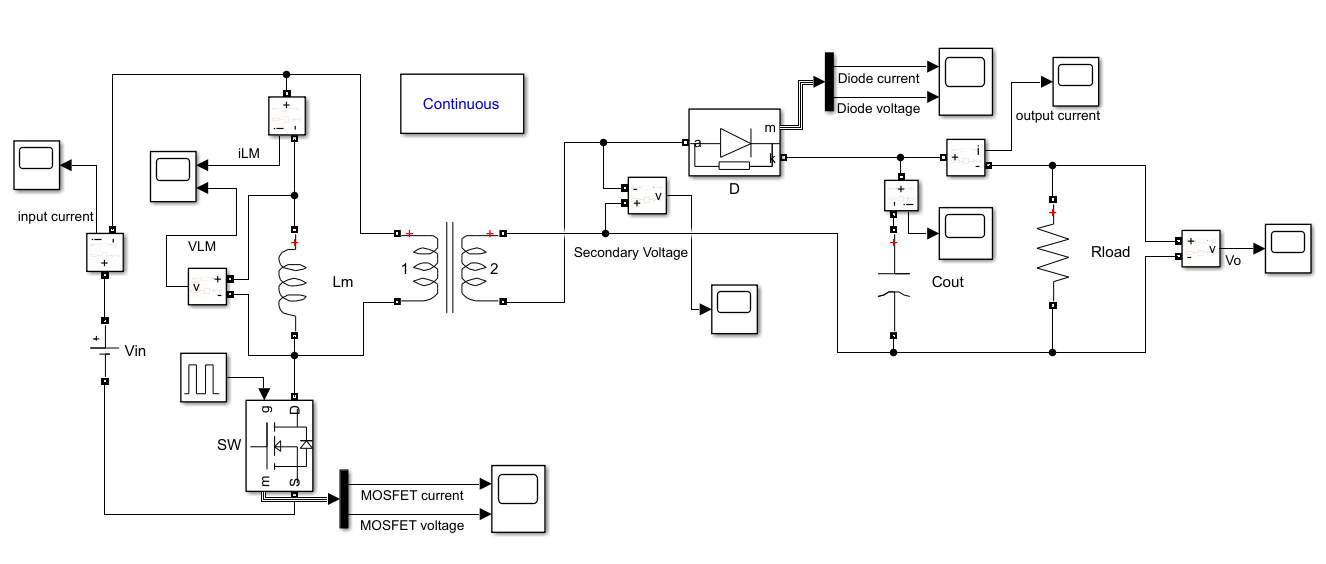
\includegraphics[width=1\textwidth]{schematic.png}
\caption{Simulink Circuit Schematic of the Flyback Converter}
\label{fig:schematic}
\end{center}
\end{figure}

\subsection{Simulation Results for $ V_{in} = 24\;V $}

The simulation results of the converter circuit for input voltage of $ V_{in} = 24\;V $ are given below.

The duty cycle of the MOSFET is determined as $ D = 5\% $ for this operation in order to keep the average output voltage at 15 V.

The duty cycle of the MOSFET is determined by some trial and errors since the converter circuit is operating in DCM. In DCM operation, the standard voltage gain equation can no more be utilized to determine the duty ratio.

The input current waveform of the converter circuit is given in Figure \ref{fig:incurr24}.

\begin{figure}[H]
\begin{center}
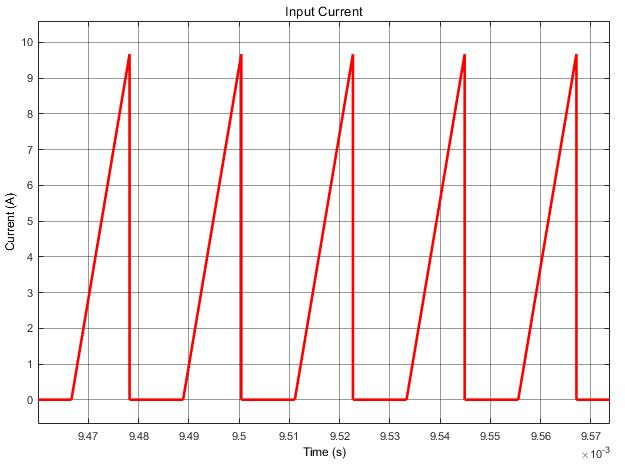
\includegraphics[width=1\textwidth]{input_current_24.jpg}
\caption{Input Current Waveform of the Flyback Converter for $ V_{in} = 24\;V $}
\label{fig:incurr24}
\end{center}
\end{figure}

The input current ripple is high as can be seen from Figure \ref{fig:incurr24} since the switch is positioned in series to the input side. The maximum current drawn from the input source and the peak to peak input current ripple is equal to 9.681 A. The high input current ripple might cause EMI effects by affecting the operation of the analog controller and gate driver circuit of the switch.

The MOSFET current and voltage waveforms of the converter circuit are given in Figure \ref{fig:mos24}.

\begin{figure}[H]
\begin{center}
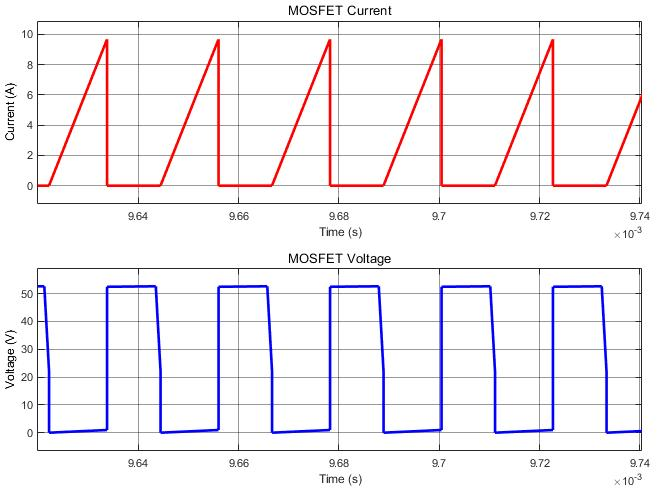
\includegraphics[width=1\textwidth]{MOSFET_curr_volt_24.jpg}
\caption{MOSFET Current and Voltage Waveforms of the Flyback Converter for $ V_{in} = 24\;V $}
\label{fig:mos24}
\end{center}
\end{figure}

The maximum current through the MOSFET during its on period is observed from Figure \ref{fig:mos24} to be 9.681 A. The maximum voltage across the switch during its off period is also observed to be 52.63 V.

The voltage and current waveforms of the magnetizing inductor of the transformer of the converter circuit are given in Figure \ref{fig:ind24}.

\begin{figure}[H]
\begin{center}
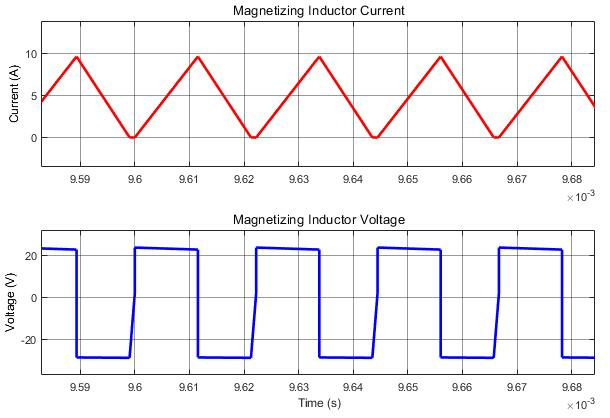
\includegraphics[width=1\textwidth]{inductor_volt_curr_24.jpg}
\caption{Magnetizing Inductor Voltage and Current Waveforms of the Flyback Converter for $ V_{in} = 24\;V $}
\label{fig:ind24}
\end{center}
\end{figure}

The DCM operation of the converter circuit can also be observed from the magnetizing inductor current waveform given in Figure \ref{fig:ind24}. It is seen from the Figure \ref{fig:ind24} that the inductor current reaches to zero and stays at zero for a finite duration until the next switching cycle.

The maximum magnetizing inductor current is observed to be equal to 9.669 A from the simulations.

The magnetizing inductor voltage switches between 24 V and -28.63 V during the switching operation.

The diode voltage and current waveforms of the converter circuit are given in Figure \ref{fig:dio24}.

\begin{figure}[H]
\begin{center}
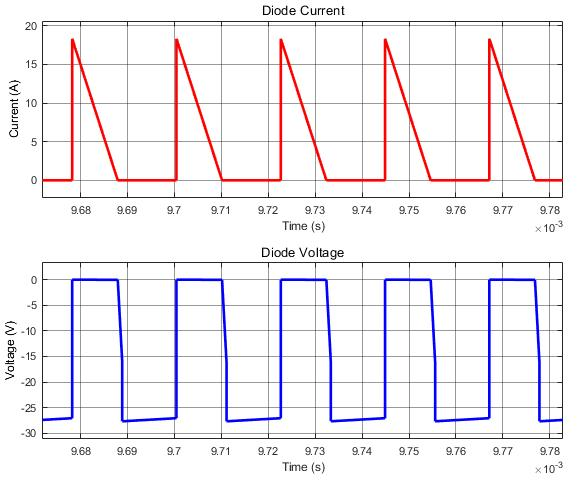
\includegraphics[width=1\textwidth]{diode_curr_volt_24.jpg}
\caption{Diode Voltage and Current Waveforms of the Flyback Converter for $ V_{in} = 24\;V $}
\label{fig:dio24}
\end{center}
\end{figure}

The voltage waveform on the secondary side of the transformer of the converter circuit is given in Figure \ref{sec24}.

\begin{figure}[H]
\begin{center}
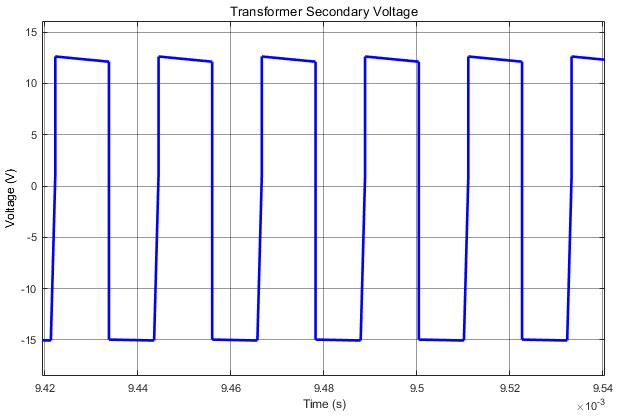
\includegraphics[width=1\textwidth]{secondary_voltage_24.jpg}
\caption{Secondary Voltage Waveform of the Transformer of the Flyback Converter for $ V_{in} = 24\;V $}
\label{fig:sec24}
\end{center}
\end{figure}

The secondary side voltage of the transformer switches between 12.63 V and -15 V during the switching operation.

The output current waveform of the converter circuit is given in Figure \ref{fig:outcurr24}.

\begin{figure}[H]
\begin{center}
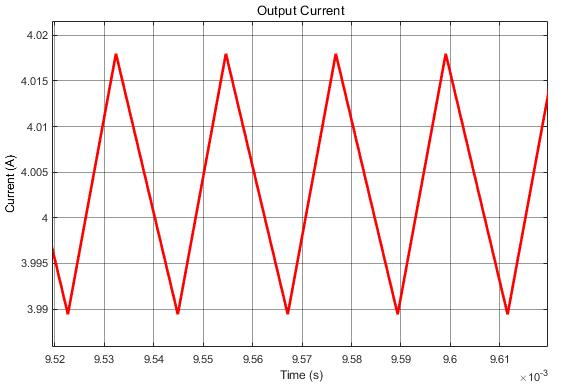
\includegraphics[width=1\textwidth]{output_current_24.jpg}
\caption{Output Current Waveform of the Flyback Converter for $ V_{in} = 24\;V $}
\label{fig:outcurr24}
\end{center}
\end{figure}

The average output current is approximately obtained as 4 A.

The output voltage waveform of the converter circuit is given in Figure \ref{fig:outvolt24}.

\begin{figure}[H]
\begin{center}
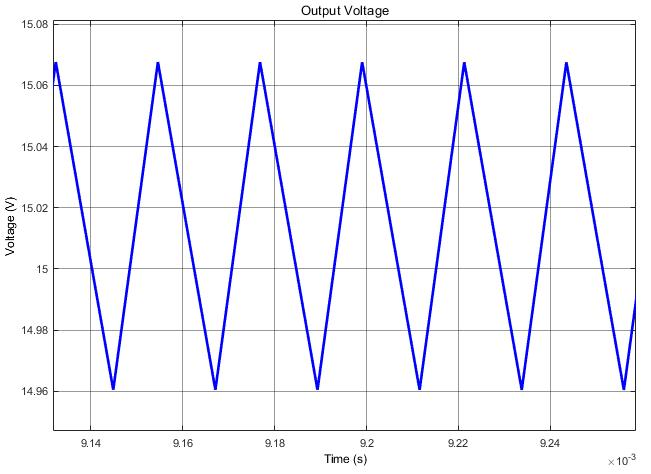
\includegraphics[width=1\textwidth]{output_voltage_24.jpg}
\caption{Output Voltage Waveform of the Flyback Converter for $ V_{in} = 24\;V $}
\label{fig:outvolt24}
\end{center}
\end{figure}

The average output voltage is obtained as 15 V as can be seen from Figure \ref{fig:outvolt24}. The peak to peak output voltage ripple is approximately equal to 0.116 V, which is less than the desired peak to peak output voltage ripple limit (4\%) of 0.6 V.

\subsection{Simulation Results for $ V_{in} = 48\;V $}

The simulation results of the converter circuit for input voltage of $ V_{in} = 48\;V $ are given below.

The duty cycle of the MOSFET is determined as $ D = 0.52\% $ for this operation in order to keep the average output voltage at 15 V.

The input current waveform of the converter circuit is given in Figure \ref{fig:incurr48}.

\begin{figure}[H]
\begin{center}
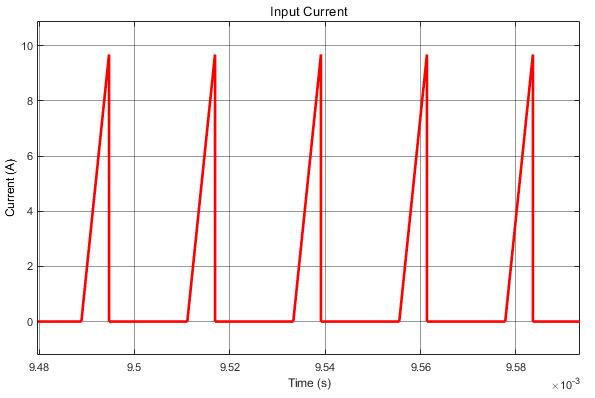
\includegraphics[width=1\textwidth]{input_current_48.jpg}
\caption{Input Current Waveform of the Flyback Converter for $ V_{in} = 48\;V $}
\label{fig:incurr48}
\end{center}
\end{figure}

Similar to the previous condition, the input current ripple is high as can be seen from Figure \ref{fig:incurr48} since the switch is positioned in series to the input side. The maximum current drawn from the input source and the peak to peak input current ripple is equal to 9.690 A. The high input current ripple might cause EMI effects by affecting the operation of the analog controller and gate driver circuit of the switch.

The MOSFET current and voltage waveforms of the converter circuit are given in Figure \ref{fig:mos48}.

\begin{figure}[H]
\begin{center}
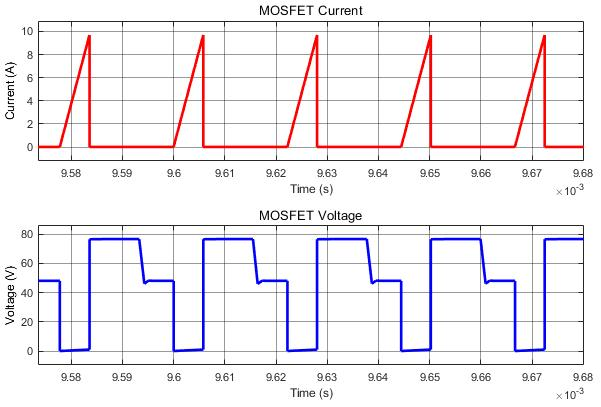
\includegraphics[width=1\textwidth]{MOSFET_curr_volt_48.jpg}
\caption{MOSFET Current and Voltage Waveforms of the Flyback Converter for $ V_{in} = 48\;V $}
\label{fig:mos48}
\end{center}
\end{figure}

The maximum current through the MOSFET during its on period is observed from Figure \ref{fig:mos48} to be 9.690 A. The maximum voltage across the switch during its off period is also observed to be 76.63 V.

It is also possible to clearly observe the DCM operation of the converter circuit from the MOSFET voltage waveform given in Figure \ref{fig:mos48}. During the off period of the switch, the voltage across the MOSFET is equal to 76.63 V until the magnetizing inductor current becomes zero. Then, until the next switching cycle (until the MOSFET becomes on again), the MOSFET voltage drops down to the input voltage ($ V_{MOSFET} = 48\;V $) and stays at this level.

The voltage and current waveforms of the magnetizing inductor of the transformer of the converter circuit are given in Figure \ref{fig:ind48}.

\begin{figure}[H]
\begin{center}
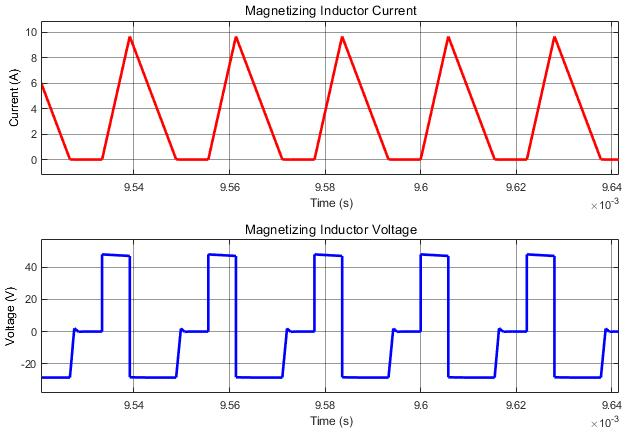
\includegraphics[width=1\textwidth]{inductor_curr_volt_48.jpg}
\caption{Magnetizing Inductor Voltage and Current Waveforms of the Flyback Converter for $ V_{in} = 48\;V $}
\label{fig:ind48}
\end{center}
\end{figure}

Again, it is also possible to observe the DCM operation from the magnetizing inductor current and voltage waveforms given in Figure \ref{fig:ind48}.

The maximum magnetizing inductor current for this operation is observed to be equal to 9.664 A.

The magnetizing inductor current discharges through the transformer and reaches to zero during the off period of the switch, and stays zero until the next switching cycle (until the MOSFET becomes on again). The magnetizing inductor voltage during that process changes from -28.63 V to 0 V when the inductor current becomes zero. During the on period of the switch, the magnetizing inductor voltage is equal to the input voltage ($ V_{inductor} = 48\;V $), and the magnetizing inductor charges linearly.

The diode voltage and current waveforms of the converter circuit are given in Figure \ref{fig:dio48}.

\begin{figure}[H]
\begin{center}
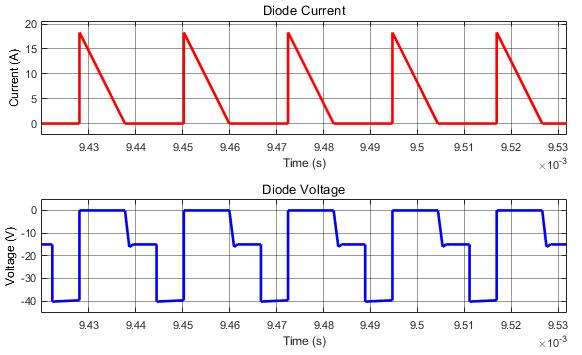
\includegraphics[width=1\textwidth]{diode_curr_volt_48.jpg}
\caption{Diode Voltage and Current Waveforms of the Flyback Converter for $ V_{in} = 48\;V $}
\label{fig:dio48}
\end{center}
\end{figure}

The DCM operation can also be clearly observed from the diode voltage waveform given in Figure \ref{fig:dio48}. During the off period of the switch, the diode stays on until the magnetizing inductor current becomes zero. Then, the diode becomes off, and stays off until the next off period of the switch. The reverse voltage across the diode during its off period changes from -15 V to -40.263 V due to this DCM operation. 

The voltage waveform on the secondary side of the transformer of the converter circuit is given in Figure \ref{sec48}.

\begin{figure}[H]
\begin{center}
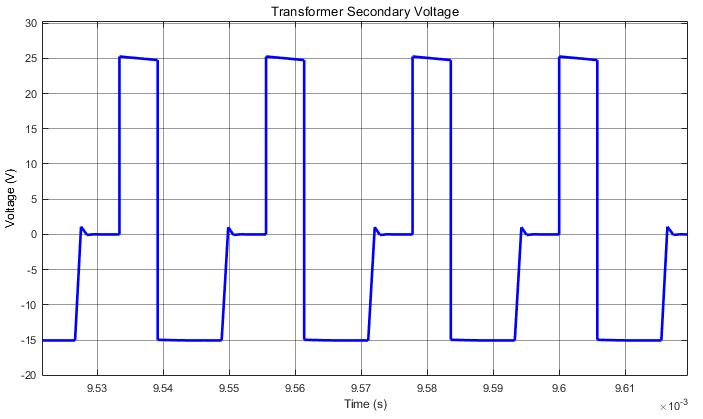
\includegraphics[width=1\textwidth]{secondary_voltage_48.jpg}
\caption{Secondary Voltage Waveform of the Transformer of the Flyback Converter for $ V_{in} = 48\;V $}
\label{fig:sec48}
\end{center}
\end{figure}

Similarly, the secondary side voltage of the transformer also exhibits some DCM behavior. During the off period of the switch, the secondary voltage is equal to the negative of the output voltage ($ V_{sec} = -15\;V $) until the magnetizing inductor current becomes zero. When the magnetizing inductor current becomes zero, the diode at the output side switches off and the secondary side voltage becomes zero.

During the on period of the switch, the magnetizing inductor charges from input. Hence, the voltage across the primary side of the transformer is equal to the input voltage ($V_{pri} = 48\;V $). As a result, the secondary side voltage becomes 25.263 V during that period due to the turn ratio between the primary and the secondary.


The output current waveform of the converter circuit is given in Figure \ref{fig:outcurr48}.

\begin{figure}[H]
\begin{center}
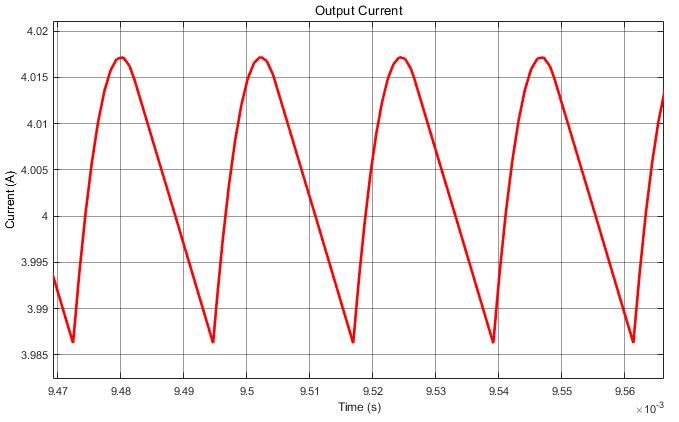
\includegraphics[width=1\textwidth]{output_current_48.jpg}
\caption{Output Current Waveform of the Flyback Converter for $ V_{in} = 48\;V $}
\label{fig:outcurr48}
\end{center}
\end{figure}

As seen from Figure \ref{fig:outcurr48} output current waveform is between 3.987 and 4.017. This current ripple is good enough for Flyback Converter. There is only resistive load, so output ripple current must be smaller than 0.15 A. In this simulation results, output current ripple is 0.03 A which is less than 0.15 Ampere.

The output voltage waveform of the converter circuit is given in Figure \ref{fig:outvolt48}.


\begin{figure}[H]
\begin{center}
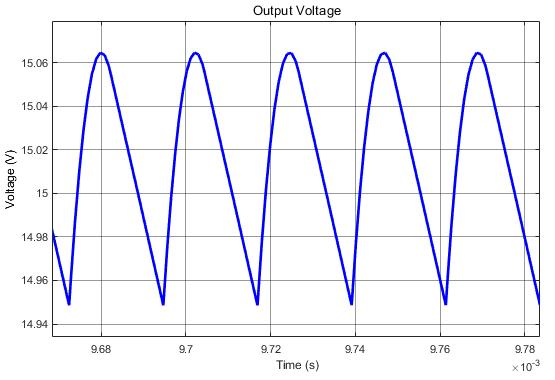
\includegraphics[width=1\textwidth]{output_voltage_48.jpg}
\caption{Output Voltage Waveform of the Flyback Converter for $ V_{in} = 48\;V $}
\label{fig:outvolt48}
\end{center}
\end{figure}

As seen from Figure \ref{fig:outvolt48}. output voltage waveform is between 15.06 and 14.96 V. Expected output voltage of e design is 15 V and output voltage ripple limit is 0.6 V. $15.06-14.96=0.1 v$ is below the design specification limits. This output voltage ripple  depends on output capacitor. 470 $\mu$F capacitor was used in simulations. Average output voltage is 15 V as expected. There is resistive load on the flyback converter thats why the shape of the output voltage is similar to the output current. Actually output voltage waveform is 3.75 times output current waveform. Output voltage waveform for 48 V input should be similar with output voltage waveform but there is differences due to different time intervals.
\section{Component Selection}
\subsection{Transformer Selection}
According to design calculations and simulation results, Peak current of the transformer 10.8 Ampere, turn ratio of the transformer is 1.9:1, primary turn number of transformer 10, secondary turn number 5, Transformer primary side voltage is between 24-48 V which is input voltage range. To obtain required turn numbers, the cross-section area of the core must be smaller than 40 $mm^2$ and core saturation density of the available cores B=1 Tesla. According to the required cross-section area range, KOOL MU 2510 E core was chosen. Cross-section area of the chosen core is 38.5 $mm^2$. Permeability of the core is given in Figure \ref{fig:Permeability}. Permeability of the KOOL MU 2510 E Core is 90$\mu$. 

\begin{figure}[!h]
\centering
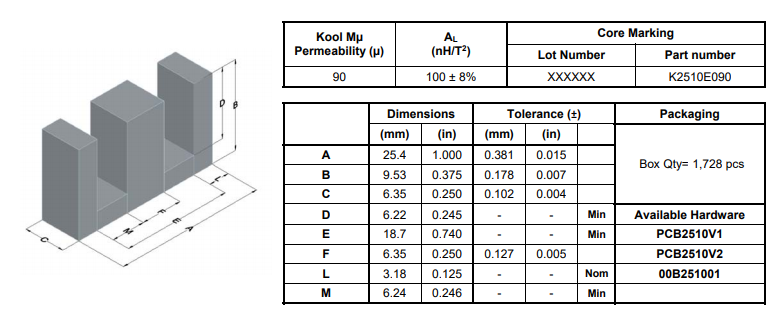
\includegraphics [width=1\textwidth]{core.png}
\caption{Detailed dimensions of the E core and relative permeability of core }
\label{fig:Permeability}
\end{figure}

The cross-section area is important to decide turn numbers and the gap between cores. Information about cross-section area and path length is given Figure \ref{fig:Csa}. As seen in (13), the gap is directly affected by path length and relative permeability, so both path length and relative permeability are also crucial for design.

\begin{align}
    gap=\frac{\mu_0\times N_P^2 \times A_e}{L_P}-\frac{l_e}{\mu_c}
\end{align}
Magnetic flux density of the core can be calculated by given formula;
\begin{align}
    B=\frac{\mu_0\times N_P\times A_e}{\frac{l_e}{\mu_c}+gap}
\end{align}

As seen from formula (14), magnetic flux density depends on the cross-sectional area, path length and relative permeability of the core. Cross-sectional area and relative permeability is limited since core can be saturated. Magnetic flux density is inversely proportional with gap and path length. As seen from Figure \ref{fig:SFD}, saturation flux density of the KOOL MU magnetic cores is 1 Tesla. Core shape, cross-section area and path length are chosen according to the saturation flux density of the KOOL MU magnetic core.

\begin{figure}[!h]
\centering
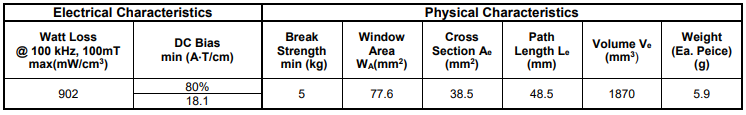
\includegraphics [width=1\textwidth]{area vs.png}
\caption{Cross section area and Path Length of core }
\label{fig:Csa}
\end{figure}
\begin{figure}[H]
\centering
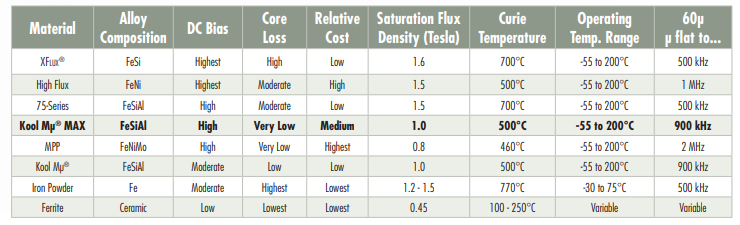
\includegraphics [width=1\textwidth]{permeability.png}
\caption{Saturation Flux Densities of various magnetic cores }
\label{fig:SFD}
\end{figure}
\subsection{Analog Controllers & Components}

Two analog controllers are used in the project for a highly flexible, efficient and feature-packed converter. The main controller is  UCC28740 Constant-Voltage Constant-Current Flyback Controller
Using Optocoupled Feedback by Texas Instruments. It will be powered by an auxiliary winding wound to the transformer. It is designated to be always used in DCM operation. It can take feedback from both primary and secondary sides and can keep output voltage constant and performs well in load and line regulation aspects. It has an embedded MOSFET driver to save space lower the component count. Furthermore, its internal algorithm also provides soft-switching to lower the initial stresses on the components.

To control synchronous switching in the secondary, UCC24636 Synchronous rectifier controller With Ultra-Low Standby current is used. It helps to replace the secondary side diode with a MOSFET to mimic its operation. As a result, the loss on diode is eliminated. Since losses on the MOSFET will be significantly lower, overall efficiency is improved. In Figure \ref{fig:refdesign2} a reference design which includes both controllers is given.

\begin{figure}[!h]
\centering
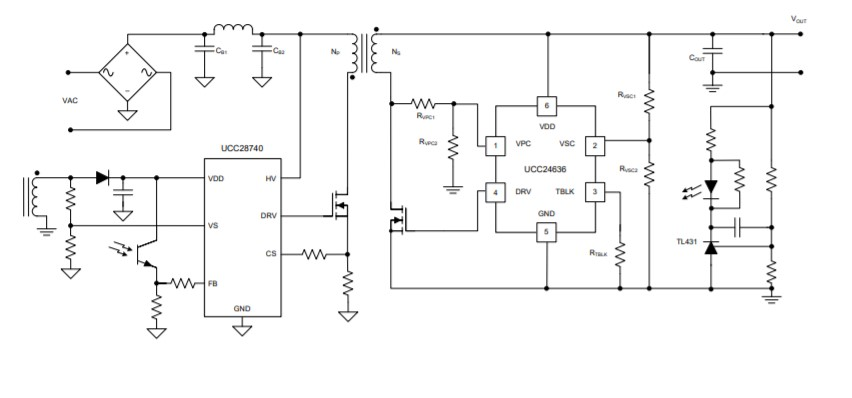
\includegraphics [width=0.6\textwidth]{refdesign2.jpg}
\caption{Flyback Controller Reference Design with UCC28749 and UCC24636}
\label{fig:refdesign2}
\end{figure}

\subsection{Cable Selection}
$\delta$= Skin Depth\\
$\rho$= Resistivity of Material\\
$\mu_r$= Relative Permeability of Cable\\
$\mu_0$= Permeability Constant = $4\pi\times 10^{-7}$
f= switching frequency = 45 kHz
\begin{align}
    \delta=\sqrt{\frac{\rho}{\pi\times f\times \mu_r\times \mu_0}}
\end{align}
Copper cable will be used in this flyback converter.
\begin{align}
\delta=\frac{7.5}{\sqrt{f}} cm   \\      \delta=\frac{7.5}{45000}=1.67\times 10^{-4} cm
\end{align}

At 45 kHz switching frequency, skin depth of copper cable is 1.67\times $10^{-4}$ cm. There is maximum 3 Ampere average current on transformer cable, so diameter of the cable must carry 3 ampere average current. To carry 3 ampere, AWG of the cable must be lower than #25 AWG. To avoid unexpected damages to our circuit, #20 AWG copper cable will be used.

\subsection{MOSFET Selection}
For the MOSFET selection, we need to consider the maximum voltage and current stresses over the MOSFET.

The maximum voltage stress over the MOSFET is obtained analytically by the following relation.

$$ V_{sw,peak} = V_{in,max} + \frac{N_P}{N_S}V_{out} $$

where $ V_{in,max} = 48\;V $, $ V_{out} = 15\;V $ and $ \frac{N_P}{N_S} = 1.9 $.

Then, the peak voltage over the MOSFET is computed analytically as follows:

$$ V_{sw,peak} = 48 + 1.9*15 = 76.5\;V $$

This value is in parallel with the peak voltage value obtained from the simulations of the Flyback Converter circuit in Simulink.

The peak voltage value for the MOSFET is obtained as $ V_{sw,peak} = 76.63 V $ from simulations.

The maximum current stress over the MOSFET is obtained analytically by the following relation.

$$ I_{sw,peak} = \frac{1}{(1-D)}\frac{N_S}{N_P}I_o + \frac{N_P}{N_S}\frac{(1-D)T_s}{2L_m}V_o $$

where $ I_o = \frac{P_o}{V_o} = \frac{60}{15} = 4\;A $

Then, the peak MOSFET current is found as follows:

$$ I_{sw,peak} = \frac{1}{(1-0.26)}*\frac{1}{1.9}*4 + 1.9*\frac{(1-0.26)*(1/45000)}{2*28.67*10^{-6}}*15 = 11\;A$$

One thing to notice here is that this peak current is computed assuming CCM operation. However, in our design, the converter mostly operates in DCM as seen from the voltage and current figures presented in the Simulation Results part. Therefore, for the MOSFET peak current value, we need to rely on the simulation results.

From the simulations of the Flyback Converter circuit in Simulink, the MOSFET peak current is observed as $ I_{sw,peak} = 9.690\;A $

Overall, the peak voltage and current ratings for the MOSFET is found as follows:

$$ V_{sw,peak} = 76.63\;V $$
$$ I_{sw,peak} = 9.690\;A $$
$$ I_{sw,mean} = \frac{I_{out}}{N_{PS}} = 2.1A $$

The selected MOSFET should also be able to handle the switching frequencies as high as 45 kHz. 
Since it is a very commonly used value, choosing a 100v MOSFET is reasonable. AOD482 by Alpha-Omega is a good choice since it is rated at 5A continuous, has a low ON resistance and costs relatively low.

\subsection{Diode Selection}
Similar to the MOSFET selection, the maximum voltage and current stresses over the diode must be determined for the diode selection.

The maximum reverse voltage across the diode during its off period can be calculated as
\begin{align*}
    V_D=V_{out}+N_{PS}V_{in,max}=-40.26V
\end{align*}
It is observed to be $ V_{diode,peak} = -40.26\;V $ from the simulations.

The maximum forward current through the diode during its on period can be calculated as:
\begin{align*}
    I_{s,peak}=\frac{2P_{out}}{D_{MAG}V_{OUT}}=18.89A
\end{align*} It is observed to be $ I_{diode,peak} = I_{s,peak} = 18.34\;A $ from the simulations.

Overall, the peak voltage and current ratings for the diode is found as follows:

$$ V_{diode,peak} = -40.26\;V $$
$$ I_{diode,peak} = 18.34\;A $$

Also, it should be noted that the average current of the diode will be equal to the output. Therefore SS5P5 from Vishay is chosen which is a Fast Recovery Schottky diode with 50V and 5A continuous rated diode which is right for the job.

\subsection{Output Capacitor Selection}
The average voltage across the output capacitor is equal to the average output voltage.

$$ V_{cap,avg} = V_{out} = 15\; $$

Then, the rated voltage of the selected capacitor must be greater than 15 V.

$$ V_{cap,rated} > 15\;V $$

One another limitation on the capacitor selection is the peak-to-peak output voltage ripple limit of the project. The peak-to-peak output voltage ripple is required to be less than 4\%.

$$ \frac{\Delta V_o }{V_o} = 0.04\;(4\%) $$

Then, the maximum allowable output voltage ripple is found as:

$$ \Delta V_o = 0.04*15\;V = 0.6\;V $$ 

Also, let's calculate the maximum allowable ESR for the required ripple.
\begin{align*}
    ESR_{C_{OUT}}=\frac{0.9V_ripple}{I_{s,max}}=20m\Omega
\end{align*}
The output voltage ripple for the Flyback Converter topology is computed from the following relation.

$$ \frac{\Delta V_o }{V_o} = \frac{DT_s}{RC} = \frac{D}{RCf_s} $$

Then, the minimum required output capacitance value is obtained as follows:

$$ C_{min} = \frac{D}{0.04*R*f_s} $$

where $ R = \frac{V_o^2}{P_o} = \frac{15^2}{60} = \frac{225}{60} = 3.75\;\ohm $

$$ C_{min} = \frac{0.26}{0.04*3.75*45000} = 77.8\;\micro F $$

Also, let's calculate the maximum allowable ESR for the required ripple.

\begin{align*}
    ESR_{C_{OUT}}=\frac{0.9V_ripple}{I_{s,max}}=20m\Omega
\end{align*}

Since it is either hard to find or very costly, using ceramic capacitors can not be used. Instead, using electrolytic capacitors in series is a good idea. However, we need to use them in parallel to reduce the ripple. Moreover, since ESR generally increases with lower capacitance a good balance needs to be found.

Using two of ESY477M025AG6AA capacitors from KEMET is a good solution. Since they have an ESR of 0.41m$\Omega$ and 470$\mu$F capacitance, they satisfy the ripple requirement.
From the simulations of the converter circuit in Simulink with the chosen output capacitor, the output voltage ripple is observed to be approximately 0.36 V, which is much lower than the maximum allowable output voltage ripple value of 0.6 V, as computed above.

The peak to peak current ripple on the output capacitor is also obtained from simulations of the converter circuit in Simulink with the chosen capacitors used. The peak to peak current ripple on the output capacitor is observed to be approximately 18.16 A.
\section{Conclusion}
\par In this report, our goal of designing a DC-DC converter as the Hardware Project of EE464 course is evaluated in detail. First, a topology for this task -Flyback Converter in our case- is chosen. Then, the main design choices and their theoretical background for Flyback Converter are discussed. After calculations, the findings are supported and verified with computer simulations. According to the obtained data, real components are chosen as a step to realize the circuit. 


\end{document}